\documentclass[tikz,border=5pt]{standalone}
\usepackage[T1]{fontenc}
\usepackage[utf8]{inputenc}
\usepackage{tikz}
\usetikzlibrary{arrows.meta,positioning,calc}

\definecolor{archdark}{HTML}{263142}
\definecolor{archslate}{HTML}{64748B}
\definecolor{stateFlex}{HTML}{C2185B}
\definecolor{stateFlexFill}{HTML}{F6D5E3}
\definecolor{stateExt}{HTML}{007C91}
\definecolor{stateExtFill}{HTML}{D5EEF2}
\definecolor{stateIdleFill}{HTML}{E5E7EB}

\begin{document}
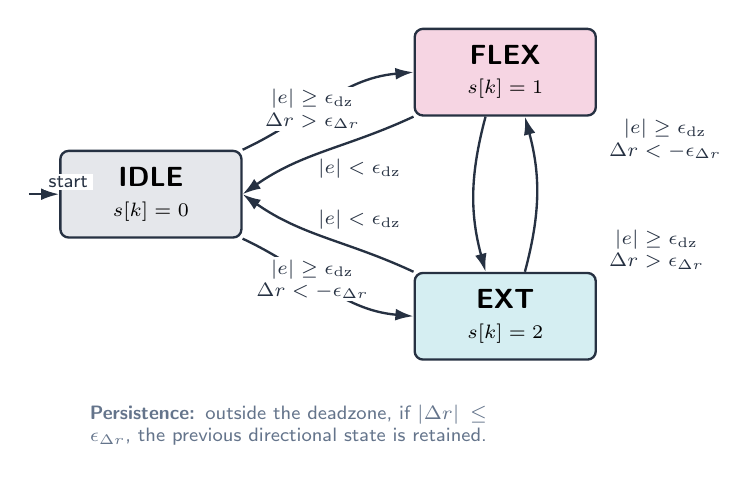
\begin{tikzpicture}[
  font=\sffamily,
  >=Latex,
  state/.style={
    draw=archdark, rounded corners=3pt, line width=0.85pt,
    minimum width=23mm, minimum height=11mm,
    inner xsep=3pt, inner ysep=2.2pt, align=center
  },
  arr/.style={-{Latex[length=2.3mm,width=1.5mm]}, line width=0.85pt, draw=archdark},
  cond/.style={font=\scriptsize\sffamily, text=archdark, fill=white,
               inner xsep=1.8pt, inner ysep=0.8pt, align=center},
  note/.style={font=\scriptsize\sffamily, text=archslate, align=left}
]

% Compact triangular state layout
\node[state, fill=stateIdleFill] (idle) at (0,0) {\textbf{IDLE}\\[-0.5mm]\scriptsize $s[k]=0$};
\node[state, fill=stateFlexFill] (flex) at (4.5,1.55) {\textbf{FLEX}\\[-0.5mm]\scriptsize $s[k]=1$};
\node[state, fill=stateExtFill] (ext) at (4.5,-1.55) {\textbf{EXT}\\[-0.5mm]\scriptsize $s[k]=2$};

% Start
\draw[arr] (-1.55,0) -- (idle.west);
\node[cond, anchor=south] at (-1.05,0.05) {start};

% IDLE -> directional request
\draw[arr] (idle.north east) to[out=25,in=185] (flex.west);
\node[cond] at (2.05,1.08) {$|e|\ge\epsilon_{\rm dz}$\\$\Delta r>\epsilon_{\Delta r}$};

\draw[arr] (idle.south east) to[out=-25,in=175] (ext.west);
\node[cond] at (2.05,-1.08) {$|e|\ge\epsilon_{\rm dz}$\\$\Delta r<-\epsilon_{\Delta r}$};

% Return to IDLE
\draw[arr] (flex.south west) to[out=205,in=35] (idle.east);
\node[cond] at (2.65,0.32) {$|e|<\epsilon_{\rm dz}$};

\draw[arr] (ext.north west) to[out=155,in=-35] (idle.east);
\node[cond] at (2.65,-0.32) {$|e|<\epsilon_{\rm dz}$};

% Direct reversal between FLEX and EXT
\draw[arr] ([xshift=-2.5mm]flex.south) to[out=-105,in=105] ([xshift=-2.5mm]ext.north);
\draw[arr] ([xshift=2.5mm]ext.north) to[out=75,in=-75] ([xshift=2.5mm]flex.south);

\node[cond, anchor=west] at (5.75,0.70) {$|e|\ge\epsilon_{\rm dz}$\\$\Delta r<-\epsilon_{\Delta r}$};
\node[cond, anchor=west] at (5.75,-0.70) {$|e|\ge\epsilon_{\rm dz}$\\$\Delta r>\epsilon_{\Delta r}$};

% Persistence rule presented once instead of self-loops
\node[note, anchor=north west, text width=5.4cm] at (-0.9,-2.55) {
\textbf{Persistence:} outside the deadzone, if $|\Delta r|\le\epsilon_{\Delta r}$, the previous directional state is retained.};

\end{tikzpicture}
\end{document}
